\chapter{Introduction}
\label{chap:Introduction}
%
\section{System and the experimental setup}
\label{sec:intro1}
%
For this experiment, we are going to identify the parameters of the Rectilinear
Control System (Model 210).
The experimental control system is comprised of the three subsystems shown in
Figure \ref{fig:dynamicalsystem}. The first of these is the electromechanical
plant which consists of the spring/mass mechanism, its actuator and sensors.
The design features a brushless DC servomotor, high resolution encoders,
adjustable masses, and reconfigurable plant type.
%
\begin{figure}[ht]
\centering
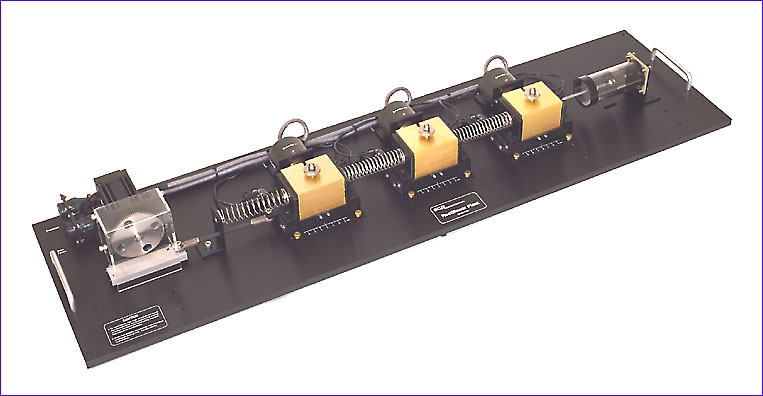
\includegraphics[width=0.8\linewidth]{linlrge}
\caption{Dynamical system}
\label{fig:dynamicalsystem}
\end{figure}
\subsection{Parameters}
The system is configured with three bodies above the mass carriage suspension
is an anti-friction ball bearing type with approximately $\pm 3$
[\si{\centi\meter}] of available travel.
The linear drive is comprised of a gear rack suspended on an anti-friction
carriage and pinion (pitch diameter 7.62 [\si{\centi\meter}]) coupled to the
brushless servo-motor shaft.
Optical encoders measure the mass carriage positions - also via a rack and
pinion with a pinion pitch about 3.18 [\si{\centi\meter}].
The bodies are connected by known stiffness springs, and a spring connects the
third mass to the frame. Instead, the first body is rigidly connected to a
pinion gear with a live-powered motor with a PC interface.
The position of each body is provided by an encoder. The position zeros are at
the equilibrium positions of the springs.
For the springs we use the nominal values provided:
%
\begin{itemize}
	\item $k_1 = k_2 = 800$ [\si{\newton\per\meter}] between $m_1$ and $m_2$, $m_2$
and $m_3$;
	\item $k_3 = 400$ [\si{\newton\per\meter}] between $m_3$ and the ground.
\end{itemize}
%
The shifts $x_1$, $x_2$, $x_3$ are provided in encoder counts, where the
relationship (\ref{eq:encodercounts}) between the measured counts and the
displacement was used.
Where $r_{e}$ is the radius of the encoder and $2\pi r_{e} = 0.0706$
[\si{\meter}]; 16000 is the number of counts per encoder revolution.
%
\begin{equation}
	\Delta x = 2\pi \cdot r_{e} \cdot \frac{\Delta count}{16000}
	\label{eq:encodercounts}
\end{equation}
%
The input data are given by the voltage \si{\volt}.
The following relation between the applied voltage and the applied force holds:
$f = (k_a \cdot k_t \cdot k_{mp}) \cdot v$.\\
Where:\begin{description}
	\item $k_a$ is the Servo Amp gain:
	\begin{equation*}
		k_a \approx 2 \quad [\text{\si{\ampere\per\volt}}]
	\end{equation*}
	\item $k_t$ is the Servo Motor Torque constant:
	\begin{equation*}
		k_t	\approx	0.1 \quad 	[\text{\si{\newton\meter\per\ampere}}]
	\end{equation*}
	\item $k_{mp}$ is the Motor Pinion pitch radius inverse:
	\begin{equation*}
		k_{mp} 	= 26.25 \quad	[\text{\si{\per\meter}}]
	\end{equation*}
\end{description}
%
\section{The dynamical model}
\label{sec:dynamicalmodel}
%
\subsection{Assumption}
\label{subsec:assumption}
The system described in the previous chapter is modelled as a linear system and
for this reason some simplifications are made.
It is considered that all the bodies move on the same axis, assuming therefore
that the rack meshed by the pinion plots the force on this axis, so that a
straight motion is assumed.
In the model there are only viscous frictions.
The block containing the engine with the attachment unit and rack is considered
rigidly connected to the mass m, according to the equation:
\begin{equation}
	\label{eq:reducedinertia}
	\begin{cases}
		m_{1} &=  m_{11} + \frac{J_{\text{motor}}}{r^2}\\
		c_{1} &=  c_{11} + \frac{c_{\text{motor}}}{r^2}
	\end{cases}
\end{equation}
In equation \eqref{eq:reducedinertia}: $r$ is the radius of the pinion-rack
coupling, $J_{\text{motor}}$ the inertia of the motor, $c_{\text{motor}}$ the
rotational damping.
While $m_{11}$ and $c_{11}$ are respectively the mass and damping of the first body.
%
\subsection{Equation of motion}
\label{subsec:equationofomotion}
We describe the equations of motion for each body according to the embodiments
reported in \eqref{eq:equationmotion}, the schematic representation is
observable in the figure \ref{fig:modelscheme}
%
\begin{equation}
	\label{eq:equationmotion}
	\begin{array}{l}
		m_1 \ddot{x}_{1} = k_1 (x_2 - x_1) - c_1 \dot{x}_{1} + g_{\text{v}} \cdot v	\\
		m_2 \ddot{x}_{2} = k_1 (x_1 - x_2) + k_2 (x_3 - x_2) - c_2 \dot{x}_{2} \\
		m_3 \ddot{x}_{3} = k_2 (x_2 - x_3) - c_3 \dot{x}_{3} - k_3 x_3	\\
	\end{array}
\end{equation}
%
The equation in matrix form is shown below (\ref{eq:matrixform}):
%
\begin{equation}
	\label{eq:matrixform}
	\begin{bmatrix}
		m_1	&  	0	&	0	\\
 		0	& 	m_2	&	0	\\
 		0	&  	0	&	m_3	\\
	\end{bmatrix}
	\ddot{x}+
	\begin{bmatrix}
		c_1	&	0	&	0	\\
  		0	&	c_2	&  	0	\\
  		0	&	0	& 	c_3	\\
	\end{bmatrix}
	\dot{x}+
	\begin{bmatrix*}[c]
		k_1		&	-k_1			&       0	\\
 		-k_1		& 	k_1 + k_2	&     -k_2	\\
  		0		&	-k_2			& k_2 + k_3	\\
	 \end{bmatrix*}
 	x=\begin{bmatrix}
 	g_{\text{v}}	\\
 	0 	\\
 	0
 	\end{bmatrix} \cdot v
\end{equation}
%
\begin{figure}[hb]
	\centering
    \resizebox{\linewidth}{!}{\begin{tikzpicture}
%\draw[help lines] (0,0) grid [step = 5 mm](15,3.5);
%\foreach \x in {0,1,...,15}
%   \draw [help lines] (\x,0) node [below,%
%          font=\footnotesize] {$\x$} -- (\x,0);
%\foreach \y in {0,1,...,3.5}
%   \draw [help lines] (0,\y) node [left,%
%          font=\footnotesize] {$\y$} -- (0,\y);

% Define style for spring
\tikzstyle{springshape}=[decoration={aspect=0.6, segment length=1.5mm, amplitude=1mm, coil}, decorate];
\newcommand{\spring}[3]{%
	% pass 3 arguments:
	% arg1: #1 coordinate x; arg2:  #2 coordiante y; arg3: #3 number of componets
	\coordinate (attachleftside) at ({#1},{#2});
	\coordinate (startspring) at ($(attachleftside) + (0.25,0)$);
	\coordinate	(endspring) at ($(startspring) + (2,0)$);
	\coordinate	(attachrightside) at ($(endspring) + (0.25,0)$);
	\draw (attachleftside) -- (startspring);
	\draw [springshape] (startspring) -- (endspring) node[draw=none,pos=0.5, above] (){$k_{#3}$};
	\draw (endspring) -- (attachrightside);
}

% Define style for dampers
\tikzstyle{dampshape}=[decoration={markings, mark connection node=dmp,
  mark=at position 0.5 with
  {
    \node (dmp) [inner sep=0pt,transform shape,rotate=-90,minimum width=15pt,minimum height=3pt,draw=none] {};
    \draw  ($(dmp.north east)+(2pt,0)$) -- (dmp.south east) -- (dmp.south west) -- ($(dmp.north west)+(2pt,0)$);
    \draw ($(dmp.north)+(0,-5pt)$) -- ($(dmp.north)+(0,5pt)$);
  }
}, decorate]
\newcommand{\dampers}[3]{%
	% pass 3 arguments:
	% arg1: #1 coordinate x; arg2: #2 coordiante y; arg3: #3 number of componets
	\coordinate (attachleftside) at ({#1},{#2});
	\coordinate (startdamp) at ($(attachleftside) + (0.25,0)$);
	\coordinate	(enddamp) at ($(startdamp) + (2,0)$);
	\coordinate	(attachrightside) at ($(enddamp) + (0.25,0)$);
	\draw (attachleftside) -- (startdamp);
	\draw [{dampshape}] (startdamp) -- (enddamp) node[draw=none,pos=0.75, above] (){$c_{#3}$};
	\draw (enddamp) -- (attachrightside);
}

% draw gear
\newcommand{\gear}[3]{%
  \def\modu{#1mm}
  \def\Zb{#2}
  \def\AngleA{#3}

  \pgfmathsetmacro{\Rpr}{\Zb*\modu/2}
  \pgfmathsetmacro{\Rb}{\Rpr*cos(\AngleA)}
  \pgfmathsetmacro{\Rt}{\Rpr+\modu}
  \pgfmathsetmacro{\Rp}{\Rpr-1.25*\modu}
  \pgfmathsetmacro{\AngleT}{pi/180*acos(\Rb/\Rt)}
  \pgfmathsetmacro{\AnglePr}{pi/180*acos(\Rb/\Rpr)}
  \pgfmathsetmacro{\demiAngle}{180/\Zb}
  \pgfmathsetmacro{\Angledecal}{(\demiAngle-2*\AnglePr)/2}

  \foreach \zz in{1,2,...,\Zb}{
    \draw
    ({(\zz))/\Zb*360-\Angledecal}:\Rb)
    -- (\zz/\Zb*360-\Angledecal:\Rp)
    to[bend right=\demiAngle]
    (\zz/\Zb*360+\Angledecal:\Rp)
    --
    plot[domain=-0:\AngleT,smooth,variable=\t]
    ({{180/pi*(-\t+tan(180/pi*\t)) +\zz/\Zb*360+\Angledecal}:\Rb/cos(180/pi*\t)})
    %
    to[bend right=\demiAngle]
    ({{180/pi*(\AngleT+tan(180/pi*-\AngleT)) +(\zz+1)/\Zb*360-\Angledecal}:
      \Rb/cos(180/pi*-\AngleT)})
    %
    plot[domain=-\AngleT:-0,smooth,variable=\t]
    ({{180/pi*(-\t+tan(180/pi*\t)) +(\zz+1)/\Zb*360-\Angledecal}:\Rb/cos(180/pi*\t)});
  }
}

% Define ground
\tikzstyle{ground}=[fill,pattern=north east lines,draw=none,minimum width=2cm,minimum height=0.3cm, rotate=90];
\tikzstyle{groundc}=[fill,pattern=north east lines,draw=none,minimum width=10mm,minimum height=0.2cm, rotate=90];
\begin{scope}[xshift=-3cm]
	\draw  (0,2.5) circle (2);
	\node [draw=none, anchor = north west] at (2,2.5) {$J_{0}$};
	\draw  (-2,0) rectangle (2,0.5);
	\draw[ultra thick] (2,0.25) -- (3,0.25);
	\draw [thick, red](1,-0.35)--(1,-0.65);
	\draw [-stealth, thick, red] (1,-0.5) -- (2,-0.5);
	\node [draw=none, anchor = north west] at (2,-0.5) {$F$};
\end{scope}
% generate plot
\begin{scope}[xshift=0cm]
	\draw (0,0) rectangle (2,1) node[draw=none,pos=0.5] () {$m_{1}$};
	\spring{2}{0.5}{1};
	\dampers{1}{2}{1};
	\draw [thick] (3.5,1.5) -- (3.5,2.5);
	\node [groundc,anchor=north]  at (3.5,2){};
	\draw [thick] (1,1) -- (1,2);
	\draw [thick, gray](1,-0.35)--(1,-0.65);
	\draw [-stealth, thick, gray] (1,-0.5) -- (2,-0.5);
	\node [draw=none, anchor = north west] at (2,-0.5) {$x_1$};
\end{scope}
\begin{scope}[xshift=4.5cm]
	\draw (0,0) rectangle (2,1) node[draw=none,pos=0.5] () {$m_{2}$};
	\spring{2}{0.5}{2};
	\dampers{1}{2}{2};
	\draw [thick] (3.5,1.5) -- (3.5,2.5);
	\node [groundc,anchor=north]  at (3.5,2){};
	\draw [thick] (1,1) -- (1,2);
	\draw [thick, gray](1,-0.35)--(1,-0.65);
	\draw [-stealth, thick, gray] (1,-0.5) -- (2,-0.5);
	\node [draw=none, anchor = north west] at (2,-0.5) {$x_2$};
\end{scope}
\begin{scope}[xshift=9cm]
	\draw (0,0) rectangle (2,1) node[draw=none,pos=0.5] () {$m_{3}$};
	\spring{2}{0.5}{3};
	\dampers{1}{2}{3};
	\draw [thick] (3.5,1.5) -- (3.5,2.5);
	\node [groundc,anchor=north]  at (3.5,2){};
	\draw [thick] (1,1) -- (1,2);
	\draw [thick] (4.5,-0.5) -- (4.5,1.5);
	\node [ground,anchor=north]  at (4.5,0.5){};
	\draw [-stealth, thick, gray] (1,-0.5) -- (2,-0.5);
	\draw [thick, gray](1,-0.35)--(1,-0.65);
	\node [draw=none, anchor = north west] at (2,-0.5) {$x_3$};
\end{scope}
\end{tikzpicture}
}
	\caption{model system}
	\label{fig:modelscheme}
\end{figure}
